%!TEX encoding = UTF-8 Unicode
%!TEX TS-program = pdflatex

%%% --- PREAMBLE --- %%%

\documentclass[a4paper,11pt]{article}

\usepackage[italian]{babel}
\usepackage[left=2cm,right=2cm,top=2cm,bottom=2cm]{geometry}
\usepackage[T1]{fontenc} % OT1: basic, T1: western, T3 and T5: exotic, T4: lots of characters but WORSE READABILITY
\usepackage[utf8x]{inputenc} % utf8x supports more characters than utf8
\usepackage{graphicx} % import PNG, JPG and PDF with \includegraphics
\usepackage[usenames,table]{xcolor} % \color
\usepackage{amssymb}
\usepackage{amsmath}
\usepackage{amsfonts}
\usepackage{float}
%\usepackage{mathtools} % (!! PLACE BEFORE hyperref !!)
%\usepackage{xfrac} % \sfrac
%\usepackage{cancel} % \cancel \cancelto
%\usepackage{hyperref} % interactive links in TOC, URLs and references
% unneded \usepackage{fixltx2e} % provides \textsubscript and makes some fixes
%\usepackage[version=3]{mhchem} % \ce (chemical formula)
\usepackage{siunitx} % \num \si \SI
%\usepackage{alltt} % {alltt} (like verbatim but with commands)
%\usepackage{moreverb} % {listing}
\usepackage{listings} % {lstlisting}
%\usepackage[overload]{textcase} % fixes \MakeUppercase and \MakeLowercase
%\usepackage[normalem]{ulem} % \uline \uwave \sout \xout
%\usepackage{enumerate} % adds options for {enumerate}
%\usepackage{paralist} % inline lists with {inparaenum}
%\usepackage[official]{eurosym} % \euro
%\usepackage{tabu} % {tabu} (like {tabular} with improvements)
%\usepackage{layout} % layout description
%\usepackage{multicol} % {multicols}
%\usepackage{lipsum} % filling text generator with \lipsum
%\usepackage[section]{placeins} % inhibits float figures from trepassing a section boundary
\usepackage{subfig} % \subfloat to be used inside {figure}
%\usepackage{wrapfig} % {wrapfigure} (like {figure} but allows text to flow on its sides)
%\usepackage{ifthen} % \ifthenelse
%\usepackage{calc}
%\usepackage{array}
%\usepackage{multirow}
\usepackage{booktabs} % \toprule, \midrule, \bottomrule

\graphicspath{ {../Figs-Tabs/} } % graphics search directories
\setcounter{tocdepth}{1} % -1: part, 0: chapter, 1: section, 2: subsection, 3: subsubsection

\lstset{ %
	language=C,
	deletekeywords={},
	morekeywords={},
	backgroundcolor=\color{white},
	basicstyle=\ttfamily\small,
	commentstyle=\color{teal},
	keywordstyle=\color{magenta},
	stringstyle=\color{purple},
	identifierstyle=\color{violet!80!black},
	numbers=left,
	numbersep=7pt,
	numberstyle=\scriptsize\sffamily\color{gray},
	stepnumber=1,
	breakatwhitespace=false,
	breaklines=true,
	keepspaces=true,
	showspaces=false,
	showstringspaces=false,
	showtabs=false,
	tabsize=2,
	captionpos=none,
}

\newcommand{\swaphmargins}{
\newlength{\tmplength}
\setlength{\tmplength}{\oddsidemargin}
\setlength{\oddsidemargin}{\evensidemargin}
\setlength{\evensidemargin}{\tmplength}}

\newcommand{\setdispacing}[1][0pt]{\setlength{\abovedisplayskip}{#1}
\setlength{\belowdisplayskip}{#1}
\setlength{\abovedisplayshortskip}{#1}
\setlength{\belowdisplayshortskip}{#1}}

\newcommand{\inv}[1]{\frac{1}{#1}}
\newcommand{\dd}{\mathrm{d}}
%\newcommand{\deriv}[2][x]{\frac{\dd #2}{\dd #1}}
%\newcommand{\derivn}[3][x]{\frac{\dd^{#2}#3}{\dd{#1}^{#2}}}
%\newcommand{\pardv}[2][x]{\frac{\partial #2}{\partial #1}}
%\newcommand{\pardvn}[3][x]{\frac{\partial^{#2}#3}{\partial{#1}^{#2}}}
%\newcommand{\integ}[2][x]{\int #2\,\dd #1}
%\newcommand{\invinteg}[2][x]{\int\frac{\dd #1}{#2}}
%\newcommand{\dinteg}[4]{\int_{#1}^{#2}#3\,\dd #4}
%\renewcommand{\arcsin}{\operatorname{asin}}
%\renewcommand{\arccos}{\operatorname{acos}}
%\renewcommand{\arctan}{\operatorname{atan}}
%\DeclareMathOperator{\arccot}{arccot}
%\newcommand{\vel}{\vee}
%\newcommand{\et}{\wedge}

%\newcommand{\fwhm}{\text{FWHM}}
%\newcommand{\hwhm}{\text{HWHM}}

\newcommand{\ndr}[1]{\footnote{#1 (n.d.r.)}}
\newcommand{\fig}[1]{figura (\ref{fig:#1})} %inserting reference to figures
\newcommand{\tab}[1]{tabella (\ref{tab:#1})} % inserting reference to tables
\newcommand{\dof}{\text{ dof}} % degrees of freedom
\newcommand{\paral}{\mathbin{\|}} % impedance parallel
\DeclareSIUnit\deca{decade} % decade unit definition for use in siunitx

% temporary, for this thing only
\newcommand{\angerr}[2]{%
	\ang{#1}{\SI[multi-part-units = repeat]{#2}{\arcminute}}
}
\newcommand{\sezione}[1]{\textsf{Sezione \ref{#1}}}
\newcommand{\figura}[1]{\textsf{Figura \ref{#1}}}
\newcommand{\tabella}[1]{\textsf{Tabella \ref{#1}}}
\newcommand{\equazione}[1]{\textsf{Equazione \ref{#1}}}

\sisetup{%
	separate-uncertainty = true,
	per-mode = symbol,
	bracket-numbers = false,
	multi-part-units = single,
	table-number-alignment = center,
	range-phrase = \text{--},
	range-units = brackets,
	output-complex-root =  \text{\ensuremath{j}},
	table-figures-decimal = 3,
	table-figures-exponent = 0,
	table-figures-integer = 2,
	table-figures-uncertainty = 2,
}

%%% --- DOCUMENT --- %%%


%%%%% SIunitX example use:
% \si{\kilo\volt\per\meter\squared} -> kV/m^2
% \SI{1.222 (34)}{\joule\second}    -> 1.222 +- 0.034 Js
% \SI{1.222 \pm 0.034}{\nF}         -> 1.222 +- 0.034 nF
% use it plz

\author{Gruppo BF \\ Roberto Ribatti, Thomas Giannoni, Valerio Lomanto}
\title{Esperienza N.2 - Ottica 1}
\date{24 Febbraio 2017}

\begin{document}
\maketitle

\begin{abstract}
L'esperienza è divisa in due parti, l'obiettivo della prima è la misura, per mezzo di uno 
spettroscopio a prisma, della lunghezza d'onda di una riga spettrale
emessa da una lampada al sodio.

Nella seconda parte si è calcolata la costante di Rydberg a partire dalla misura della lunghezza d'onda di alcune righe spettrali di emissione di una lampada all'idrogeno,m stavolta con l'uso di uno spettroscopio a reticolo. 

Si è quindi valutata la risoluzione dello strumento attraverso la misura della separazione del doppietto giallo nell'emissione della lampada al sodio.

\end{abstract}

\newpage
\part{Misura della lunghezza d'onda della riga gialla del sodio}
\section{Finalità}
	In questa parte dell'esperienza abbiamo determinato la lunghezza d’onda $\lambda_{\text{Na}}$ della riga spettrale
	emessa da una lampada al sodio.
\section{Strumentazione}\label{sez:str_a}
	La strumentazione impiegata in questa sezione è uno spettrometro a
	prisma,riportato in \textbf{figura 1};
	tale spettroscopio si compone di:
	\begin{list}{$\cdot$}{}
		\item \textbf{una sorgente } ovvero una lampada al cadmio in fase
		di
		calibrazione e una lampada al sodio in fase di misura.
		\item \textbf{due telescopi}, uno fisso, per raccogliere la luce
		della
		sorgente e inviarla sul prisma, ed un telescopio di osservazione
		montato su di un piatto rotante e dotato di goniometro
		(sensibilità di $1/60$ di grado), in grado di ruotare
		rispetto al prisma.
		Il telescopio di raccolta  è munito di una fenditura regolabile
		attraverso la quale regolare l'ingresso della luce.

		Il telescopio di osservazione permette la regolazione del fuoco
		ed è
		inoltre regolabile attraverso delle viti.
		\item \textbf{un prisma} che costituisce l'elemento dispersivo
		dello
		spettroscopio
	\end{list}
	\bigskip
	si è inoltre impiegata una lente di ingrandimento per facilitare la
	lettura della scala del goniometro.

	\bigskip


	\begin{figure} [h]
		\centering
		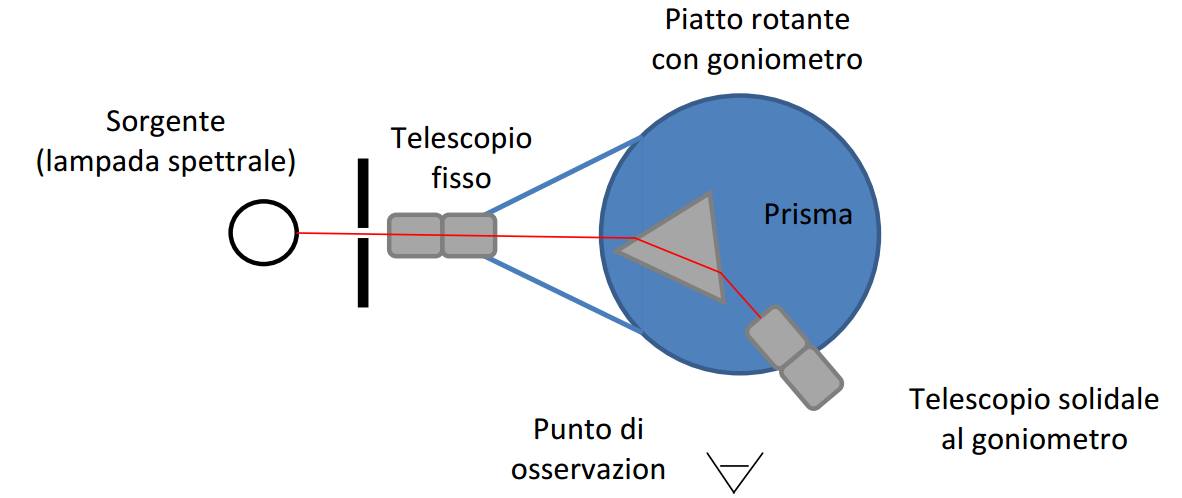
\includegraphics[width=0.9\textwidth]{./prisma}
		\caption{Schema dell'apparato impiegato.}
		\label{fig:prisma}
	\end{figure}
	Si riporta in \textbf{figura \ref{fig:prisma}} uno schema
	dell'apparato
	sperimentale impiegato.

\section{Svolgimento delle misure}
	La nostra misurazione si compone di due diverse
	fasi: una fase di calibrazione
	dell'apparato ed una fase in cui vengono
	effettuate la misure per determinare $\lambda_{\text{Na}}$.
\subsection{Calibrazione con lampada al cadmio}
	La prima fase consiste nell'azzeramento del dispositivo;
	per fare ciò abbiamo rimosso il prisma ed allineato la
	fenditura di uscita della sorgente,la fessura della slitta
	ed il reticolo a croce del telescopio di osservazione.
	Per effettuare tale allineamento sono state impiegate
	le viti per effettuare spostamenti fini di cui è dotato il piatto
	rotante.

	Abbiamo assunto la lettura del goniometro
	$\alpha_0$ quale zero di riferimento per le successive misure.
	Essendo tale misura basilare per le osservazioni successive
	abbiamo iterato tale misurazione più volte
	ottenendo $\alpha_0 = \angerr{0}{0(1)}$
	Effettuato questo primo step abbiamo reinserito il
	prisma orientandolo in maniera che formi un angolo
	di circa \ang{60}.

	Si è ruotato il telescopio di osservazione fino ad osservare
	tutte le righe nel visibile emesse dalla nostra sorgente, la lampada al
	cadmio.
	Ruotando a sua volte il prisma si osserva che le righe si spostano:
	si è bloccato il prisma all'angolo di inversione della direzione di spostamento
	della riga verde (che corrisponderebbe alla condizione di minima deviazione
	per quella riga);
	l'emissione più vicina in lunghezza d'onda a quella che
	intendiamo misurare sarebbe la riga rossa, ma riteniamo che scegliendo una
	riga meno lontana dalle altre righe del cadmio si ottenga una calibrazione migliore.
	Si sono dunque misurate le varie posizioni angolari
	delle righe di emissione della lampada al cadmio.

	\begin{table}[hb]
		\centering
		\begin{tabular}{S[%
			table-figures-decimal = 1,
			table-figures-integer = 3,
			table-figures-uncertainty = 0] r}
			\toprule
			{$\lambda $ [\si{\nm}]} & $ \alpha - \alpha_0 $ \\
			\midrule
			643.8 & \angerr{47}{49 (2)} \\
			508.6 & \angerr{49}{4 (2)} \\
			480.0 & \angerr{49}{31 (2)} \\
			467.8 & \angerr{49}{44 (2)} \\
			441.6 & \angerr{50}{18 (2)} \\
			\bottomrule
		\end{tabular}
		\caption{Posizione angolari delle righe di emissione.}
		\label{tab:disper_angolare}
	\end{table}

	Nel grafico in \fig{fit_a} si è riportata la posizione angolare contro l'inverso della
	lunghezza d'onda per poi verificarne l'andamento lineare con un fit a
	due parametri $\alpha = m \inv{\lambda} + q $.

	\begin{figure} [h]
		\centering
		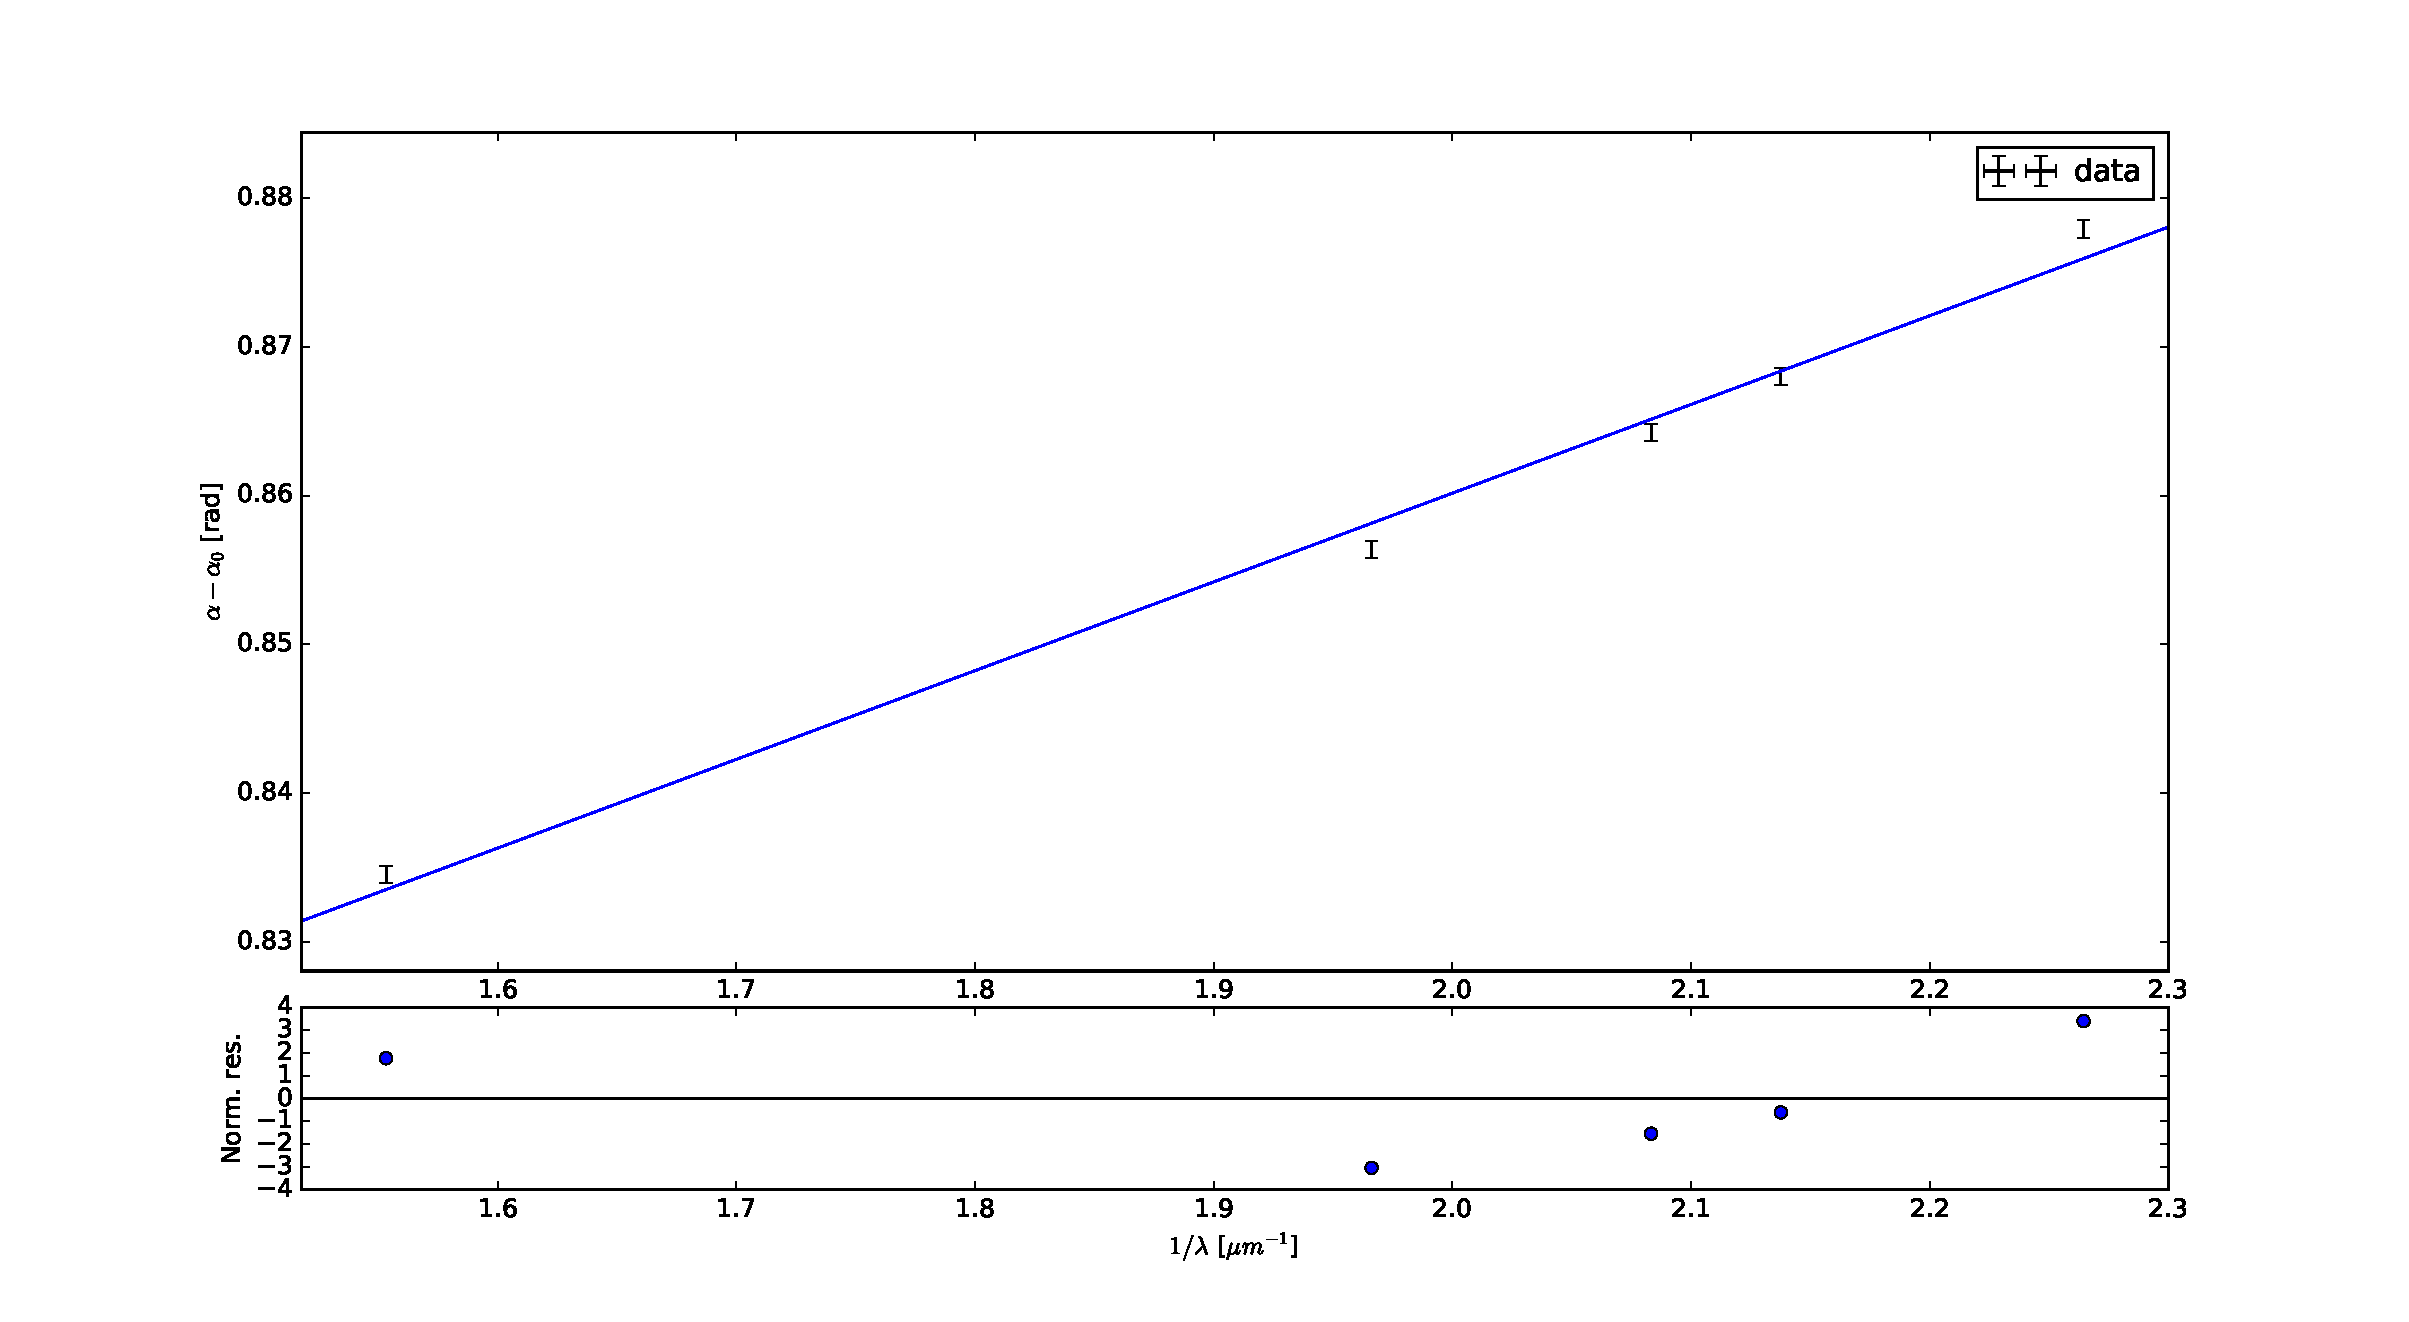
\includegraphics[scale=0.4]{fit_parteA.pdf}
		\caption{Posizione angolare contro $1/\lambda$ per le righe del cadmio e fit lineare.}
		\label{fig:fit_a}
	\end{figure}

	Il fit ha dato i seguenti valori: \\
	$m = \SI{0.0596 \pm 0.0011}{\radian\um}$ \\
	$q = \SI{0.7409 \pm 0.0022}{\radian}$ \\
	$\chi^2 = 11.8 \ (3 \dof , \  p = 0.0079) $ \\
	Con un coefficiente di correlazione di -0.992. L'alto $\chi^2$ è probabilmente
	dovuto al fatto che, a rigore, la condizione di minima deviazione vale solo
	per una delle righe spettrali misurate (quella verde), dunque non ci attendiamo
	che la relazione lineare sia esattamente verificata.

\subsection{Misura con lampada al sodio}
	Per effettuare le misure vere e proprie abbiamo
	rimontato la lampada al sodio in luogo di quella al cadmio.
	Dopo aver aspettato alcuni minuti, ritenuti necessari per la
	termalizzazione della sorgente, abbiamo osservato la posizione angolare
	$\alpha_{\text{Na}} = \angerr{48}{13(2)}$ della riga gialla del sodio.
	Dalla relazione tra quest'ultima e la lunghezza d'onda, utilizzando i parametri
	ottenuti attraverso il fit di calibrazione possiamo ricavare (tenuto conto
	anche della covarianza per la propagazione dell'errore):

	\begin{equation}
		\lambda_{\text{Na}} = \frac{m}{\alpha_{\text{Na}} - q} = \SI{592 (5)}{\nm}
	\end{equation}
	A fronte di un valore atteso di \SI{589}{\nm}, in ottimo accordo con quanto da noi misurato.

% \section{note e osservazioni}
In questa sezione la nostra principale difficoltà
è stata associare una tolleranza alle misure fatte
per ovviare a tale ognuna delle misure fatte è
stata iterata pi volte al fine di fare statistica.
 
\part{Misura della costante di Rydberg}
\section{scopo e finalità}
	In questa parte di esperienza ci proponiamo dapprima di misurare la 
	risoluzione dello spettroscopio a reticolo in dotazione;
	e successivamente la misura della costante di Rydberg.
\section{strumentazione}
	La strumentazione impiegata 
	in questa sezione risulta analoga a quella impiega
	nella \sezione{sez:str_a}.
	Si è impiegato infatti uno spettrometro a reticolo.
	Tale spettroscopio si compone di:
	\begin{list}{$\cdot$}{}
		\item \textbf{una sorgente } ovvero una lampada al mercurio in fase di
		calibrazione, una lampada al sodio ,utilizzata per controllare la risoluzione dello strumento, e per effettare la misura di Rydberg
		una lampada al idrogeno.
		\item \textbf{due telescopi}, uno fisso	,per raccogliere la luce della 
		sorgente e inviarla sul reticolo, ed un telescopio di osservazione
		montato su di un piatto rotante e dotato di goniometro 
		(sensibilità di $1/120$ di grado),in grado di ruotare 
		rispetto al prisma.
		Il telescopio di raccolta  è munito di una fenditura regolabile
		attraverso la quale regolare l'ingresso della luce.
	
		Il telescopio di osservazione permette la regolazione del fuoco ed è 
		inoltre regolabile attraverso delle viti.
		\item \textbf{un prisma} che costituisce l'elemento dispersivo dello
		spettroscopio 
	\end{list}
	\bigskip
	si è inoltre impiegato una lente di ingrandimento per facilitare la lettura della scala del goniometro.

\bigskip


\begin{figure} [!h]
	\centering
	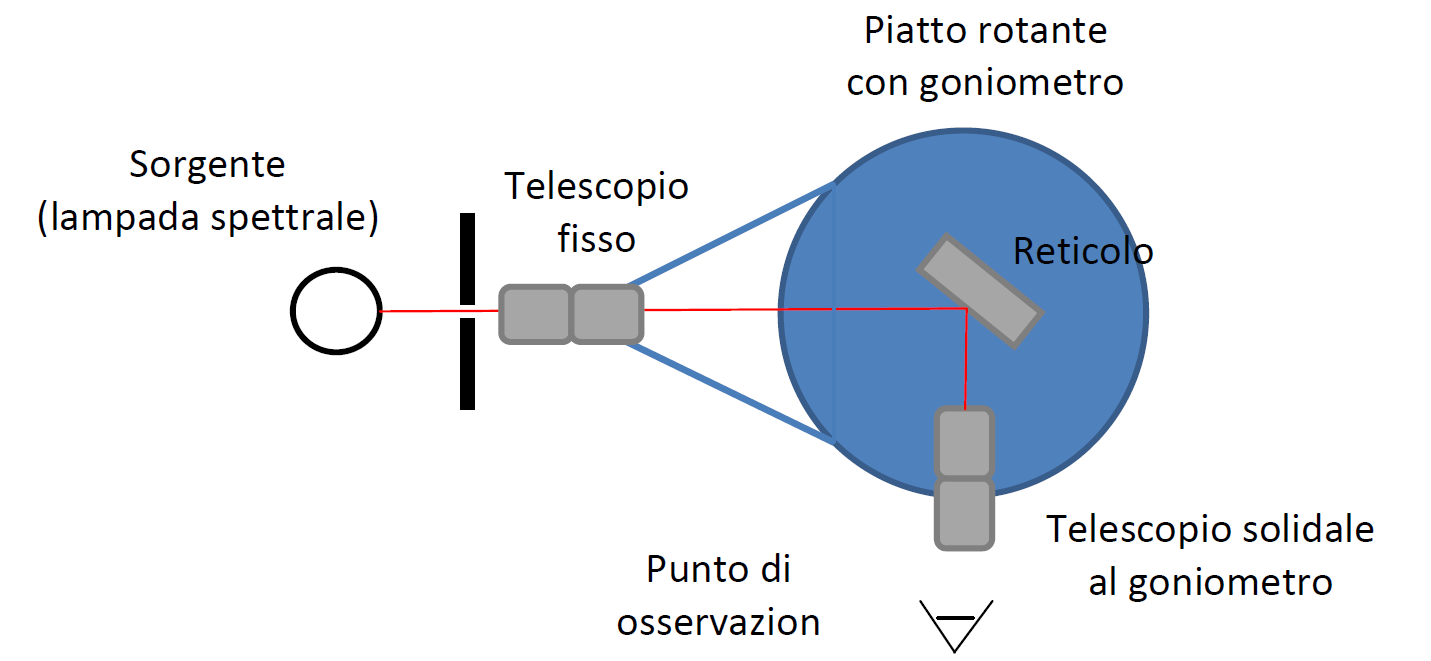
\includegraphics[width=0.9\textwidth]{./reticolo}
	\caption{Schema dell'apparato impiegato.}
	\label{fig:reticolo}
\end{figure}
Si riporta in \textbf{figura \ref{fig:reticolo} }uno schema dell'apparato
sperimentale impiegato. 
\section{Calibrazione}
	L'obiettivo della calibrazione è misurare lo "zero" del goniometro e il passo del reticolo di diffrazione.
	
	Si è montata la lampada al mercurio e si è proceduto come nella parte precedente:
	si è rimosso il reticolo e si sono allineate sorgente, fessura di ingresso del telescopio di raccolta
	ed il reticolo a croce del telescopio di osservazione.
	
	Abbiamo assunto la lettura del goniometro
	$\alpha_0$ quale zero di riferimento per le successive misure.
	Essendo tale misura basilare per le osservazioni successive la stessa è stata ripetuta da ogni membro del gruppo,
	ottenendo la stima finale di $\alpha_0 = \ang{171;21; } \pm 3' $.
	
	Si è quindi reinserito il reticolo ad un angolo $\sim \ang{60}$
	tra normale e fascio incidente.

	Per misurare il passo del reticolo si è misurato l'angolo di riflessione (ordine zero) della della sorgente sul reticolo e successivamente la riga di emissione principale del mercurio (verde) al 
	primo e secondo ordine di diffrazione. La lunghezza d'onda è nota essere $\lambda = \SI{546.074}{\nano\meter}$,
	ottenendo rispettivamente $\alpha_0=\ang{58;24;} \pm 6'$, $\alpha_1=\ang{105;55;}\pm 6"$ e $\alpha_2=\ang{144;32;}\pm 6"$.
	
	Essendo nota la relazione:
	\smallskip
	\begin{equation*}
	d\bigl(sin (\alpha_i) - sin (\alpha_d)\bigr) = m \lambda\qquad \text{con}\qquad \theta_i=\frac{1}{2}(\pi- \alpha_0)\qquad \alpha_i=(\pi- \theta_1-\alpha_m)
	\end{equation*}
	Dove per gli angoli si è seguita la notazione usata in \figurename{ \ref{fig:angoli}}.
	\bigskip
	\begin{figure} [H]
		\centering
		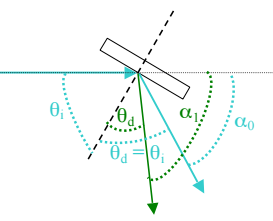
\includegraphics[width=0.4\textwidth]{../FIgs-tabs/angoli.png}
		\caption{Schema della convenzioni degli angoli impiegata.}
		\label{fig:angoli}
	\end{figure}
	\smallskip

È quindi possibile ricavare il passo reticolare $d=	\SI{84.27 \pm 0.08}{\micro\meter}$.

\section{Misura della costante di Rydberg}
	Si è sostituita la lampada al mercurio con quella all'idrogeno e si è proceduto alla misura delle righe osservabili e dell'ordine zero di riflessione.
	
	Le misure effettuate e le lunghezza d'onda ricavate sono riportate di seguito:
	\smallskip
	\begin{table}[H]
	\centering
		\begin{tabular}{c|c|c|c}
			riga & ordine & $\alpha _{m}$ & $\lambda \;\text{(nm)}$ \\
		\hline
		& $ 0 $ &$\ang{58;17;} \pm 6' $ &\\
		\hline
		blu (\SI{434.1}{\nano\meter})& $ 1 $ &$\ang{97;54;30} \pm 6' $ & $430.7 \pm 0.9$\\
		\hline
		 & $ 2$ & $\ang{128;12;} \pm 6' $ &$434.4 \pm 0.6$\\
		\hline
		verde (\SI{486.1}{\nano\meter}) & $ 1$ & $\ang{101;42;} \pm 6' $ &$483.5 \pm 1.0$\\
		\hline
		 &$ 2$ & $\ang{135;37;30} \pm 6' $&$487.6 \pm 0.6$ \\
		\hline
		rosso (\SI{656.3}{\nano\meter})&$1$ & $\ang{113;36;30} \pm 6' $ &$654.6 \pm 1.1$\\
		\end{tabular}
	\end{table}
	\smallskip

	Impiegando la nota relazione:
	\smallskip
	\begin{equation*}\label{eq:ryd}
	\frac{1}{\lambda}=R\;\biggl(\frac{1}{{n_1}^2}-\frac{1}{{n_2}^2}\biggr)
		\smallskip
	\end{equation*}

si può eseguire un fit per la costante di Rydberg, ottenendo:
$$R= \SI{1.0979\pm0.0008e7}{\meter^{-1}} \qquad \chi^2/ndof = 19/4$$ che è in ottimo accordo con il valore noto $R= \SI{1.0974e7}{\meter^{-1}}$. 

Di seguito è riportato il grafico del fit eseguito.

	\begin{figure} [H]
		\centering
		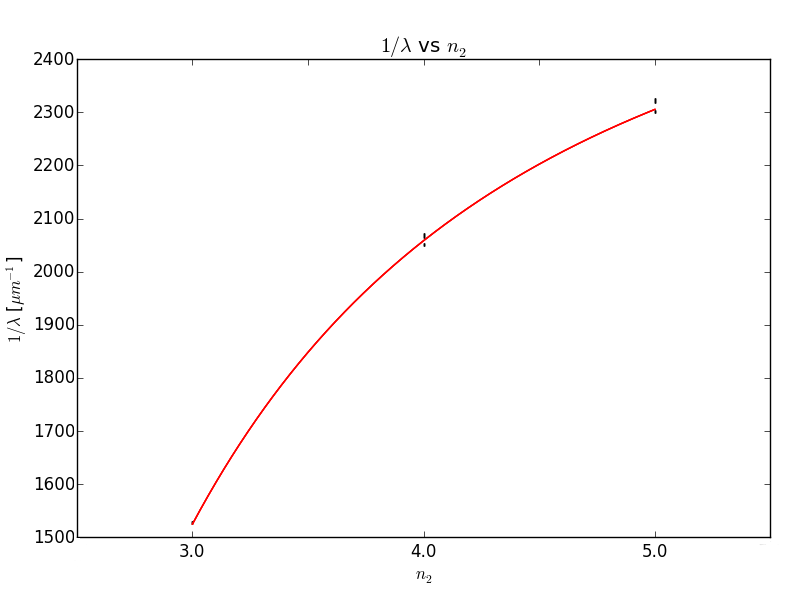
\includegraphics[width=0.8\textwidth]{../FIgs-tabs/fit_R.png}
		\caption{Fit della costante di Rydberg}
	\end{figure}

\section{Stima della risoluzione dello spettroscopio}
	Per effettuare una stima della sensibilità dello
	spettroscopio si è montata come sorgente la 
	lampada al sodio e si è misurata la posizione angolare delle righe del doppietto giallo
	del sodio, ottenendo $$\alpha_0= \ang{57;57;} \pm 6'
	\text{, }\alpha_1=	\ang{108;56;}\pm 6' \text{ e } \Delta\alpha=2' \pm 1'$$
rispettivamente l'angolo di riflessione, l'angolo della prima riga del doppietto e la distanza angolare dalla seconda.
Per la lunghezza d'onda delle due righe si ottiene:
	$$\lambda_1= \SI{589.8 \pm 1.1}{\nano\meter}\text{ e } \lambda_2=  \SI{590.3 \pm 1.0}{\nano\meter}$$
	Tali misure risultano in accordo con 
	la misura effettuata con l'apparato della prima parte e con il valore atteso di $\lambda_1^{exp}= \SI{589.0}{\nano\meter}\text{ e } \lambda_2^{exp}=  \SI{589.6}{\nm}$.
		La larghezza del doppietto misurata risulta essere $\Delta 	\lambda=\SI{0.48 \pm 0.24}{\nano\meter}$ che è compatibile con quella attesa $\Delta 	\lambda^{exp}=\SI{0.6}{\nano\meter}$.
%\section{Note}




\end{document}
